\chapter{Results and analysis}
\label{results_analysis}

Given that this research is to be continued in the following months, this report must be considered as an intermediate stage. Still, some coherent results have been found and, more importantly some of the side problems have been explained and mitigated within our means.

For the sake of clarity, this section is going to be presented in a mostly chronological way (with a final summary of the results). This will allow us to present the problems, solutions and results in a logical way.

Luckily, once the device was built and with an almost constant supply of cells (contamination issues aside), experiments are quite fast and we have been able to run close to $100$ of them.

We want to quickly recall the aim of our experiments and the protocol followed in each of them. Regarding the aim, we intend to study the influence of Chlamydomonas reinhardtii on the diffusion of micrometric tracers in a 2-dimensional environment. Concerning the protocol, we first prepare an aliquot of the algae in their medium (higher levels of concentration are achieved by centrifugation). Then, we add the tracers and, if required, the surfactant. Some wet cotton is to be put in the box if we want to prevent evaporation. We \textit{close} the device (approaching its threads) and, with the help of a pipette, we put a droplet of the desired volume between the threads, touching them. With the help of the device, we pull the threads $6 \; \textrm{mm}$ away, so as to have a thin square film, and we cover the box. Finally we turn the box upside down and we put it under the microscope, where we will wait for it to reach the expected thickness. Then we acquire images for approximately 1 minute. One of the resulting images can be seen on Fig. \ref{frame_e3}

\begin{figure}[H]
	\centering
	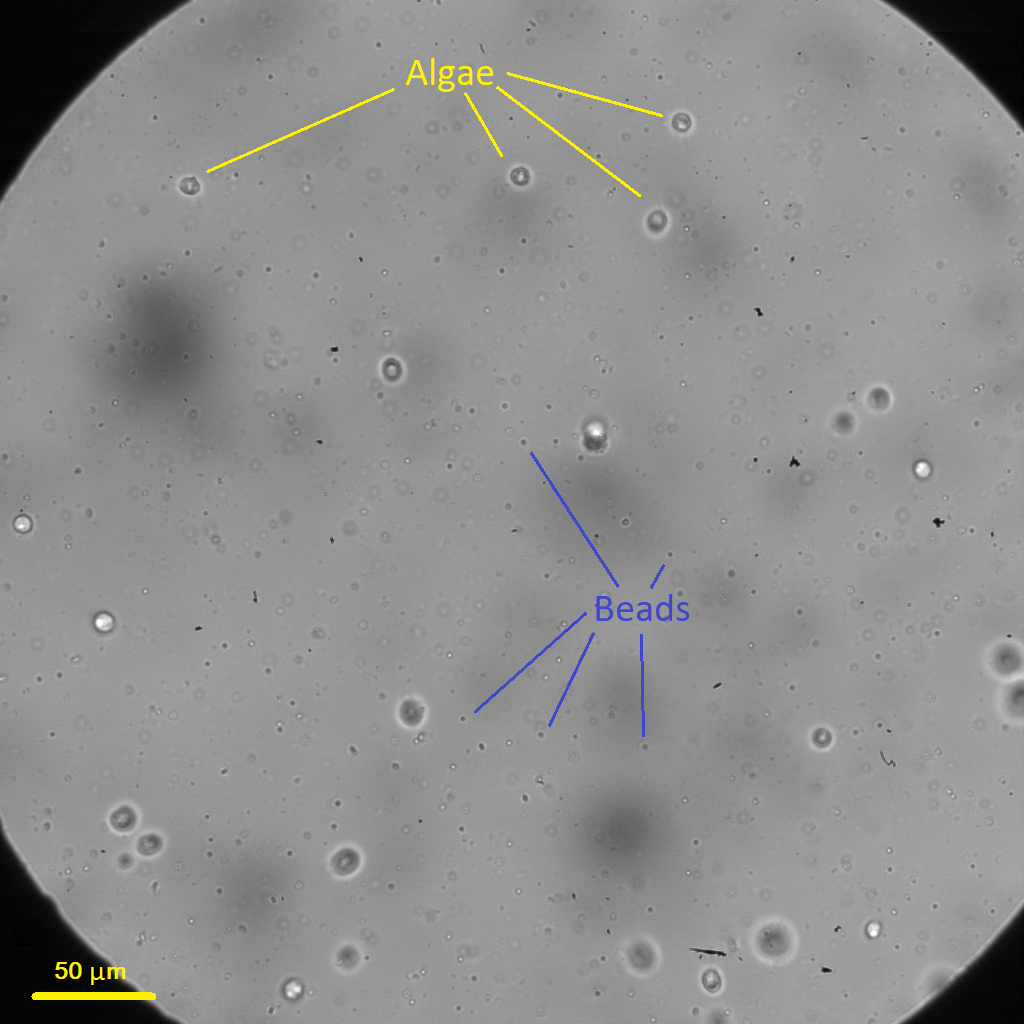
\includegraphics[width=0.65\textwidth]{archivos/e3_randomframe.png}
	\caption{Example of the frames obtained throughout the experiments}
	\label{frame_e3}
\end{figure}

As it has been explained in section ¿¿¿5.1???, diffusion can be quantified by measuring the MSD of tracers as a function of the elapsed time. This is why, in our images, we will look for the displacements, $\Delta x$ and $\Delta y$, of the tracers along the axes of the selected reference frame (usually the laboratory reference frame) for different elapsed times, $\Delta t$.

Among our experiments, most were devoted to assess the diffusion of tracers in the presence of \textit{Chlamydomonas reinhardtii}. However, a non-negligible amount of them had other purposes such as evaluating the effects of evaporation, surfactants, tilt,... This already reduces the number of available data, but much more importantly, we have not been able of exploiting most of the images satisfactorily.

The first and main reason for this is the presence of \textit{background flows}. Afterwards, as a consequence of the implemented solutions further problems arose such as the premature death of algae or the presence of quiescent beads on the surfaces of our film.

\section{Background flow}

We call \textit{background flow} to currents whose origin is unrelated to the presence of the algae. An example of this flow is shown on Fig. \ref{backg_flow}.

If the background flow were uniform, we could think of simply removing its mean numerically, but it is not the case as one can see from the figure above. 

This led us to two possibilities: either developing more complex data processing or trying to improve our experiment. 

\begin{figure}[H]
	\centering
	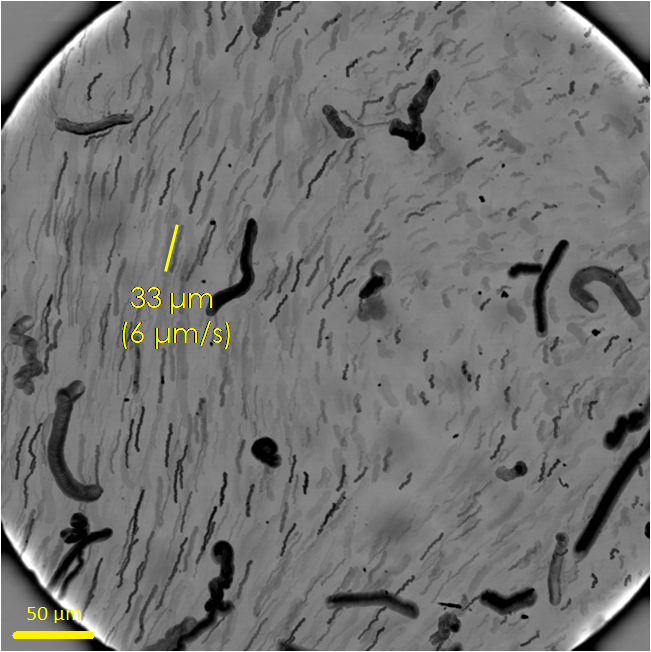
\includegraphics[width=0.65\textwidth]{archivos/backg_flow.png}
	\caption{The common trend of the streamlines (over 5.5 seconds) in the left part of the image suggests the presence of a background flow. It reflects a velocity magnitude of the order of $6 \mu m / s$}
	\label{backg_flow}
\end{figure}

\subsection{Experimental removal}

To remove this flow experimentally, we first need a better understanding of what is going on. Several hypothesis were proposed:

\begin{itemize}
	\item Evaporation
	\item Convection
	\item Marangoni stresses
	\item Tilt of the device
\end{itemize}

Since our setup had already been used by several authors in their articles, one of our first steps was to contact one of them: Dr. Jeffrey S. Guasto. Here are some of the pieces of advice he gave us in answer to our questions and our reactions to them:

\begin{itemize}
	\item \textit{We did not have a major problem with background flows. But depending on what you are looking at and length scale of the background flow, you could consider subtracting the mean from your flow of interest.}
\end{itemize}

We will consider this and other options for numerically removing the background flow in the next section.

\begin{itemize}
	\item \textit{Thin films are fundamentally quite temperamental: related to Stokes' paradox where perturbations can be quite long ranged, and actually the over side length of the film can play an important role in its behavior (not just the thickness).}
\end{itemize}

It would probably take another research project to properly analyze the effects of our boundary conditions on our problem. This is the reason why we opted for a more empiric approach, choosing the size of our layer based on previous works, such as Guasto's himself. Our film is a $6mm$ side square, whereas his is $5mm$, so this should not be a problem.

\begin{itemize}
	\item \textit{Regarding our chamber and setup: We used a similar method of humidifying the chamber to help prevent evaporation. We also blocked as many openings from the top of the sample holder and the bottom side (i.e. opening in the stage where the objective protrudes). We tried to make this enclosure as small as possible - ours measured approximately 5cm x 5cm x 5mm. The small size helps to maintain humidity and also to prevent air circulation inside of the chamber (e.g. natural convection due to slight heating). For the light source, you should aim to minimize the illumination power and of course if working with Chlamy, short wavelengths should be cut from the spectrum to avoid inadvertent phototaxis - this also helps to prevent heating though.}
\end{itemize}

The humidifying method we use consists in putting a wet cotton at the bottom of the box. 

By using a Petri dish, we managed to place the film close enough to the top cover so to have it within the \textcolor{red}{¿¿¿ focal range ???}, avoiding the need for an extra opening. 

The Petri dish inner diameter is $\phi = 5 \; \textrm{cm}$ and its height is $h = 1.3 \; \textrm{cm}$. This means our volume is $\sim 2$ times theirs, but further diminishing the height of the box does not seem to improve our situation.

Concerning the light source, we work with the minimum intensity of light allowing to obtain clear images of the algae and the tracers. We use as well a red filter to avoid phototaxis. Indeed, longer wavelengths are less energetic and the heating should be less intense. 

\begin{itemize}
	\item \textit{Regarding the fluid (...), we found that the cells were very sensitive to the surfactant concentration, and thus we minimized the concentration to ensure their motility in spite of any benefits to the film mechanics. I think that we found a concentration right around the CMC \footnote{Critical micelle concentration defined as the concentration of surfactants above which micelles are spontaneously formed~\cite{Sheng2011}} for Tween 20 worked best to maintain both the film and the cell motility. To properly control surfactant concentration - if using commercially available tracer particles - it is also critical to wash the tracers and remove the harsh surfactants in which they are packed (again for the sake of the cells).}
\end{itemize}

For the first tests without algae but with beads, we used SDS to help maintain the film, but shortly after we noticed that there was no need for it, since our layers were relatively easily formed and remained there long enough.

Based on Guasto's advice, we started washing the tracers, and even the algae, right before the experiments, to make sure the concentration of surfactants was as low as possible. The problem is that traces are always present and even the slightest concentrations can have important effects as we will see later.

So, at a certain point, we also decided to try and use Tween 20 in some of our experiments to reproduce Guasto's experiment as accurately as possible, since he did not find such problems. This does not seem to work though.

\begin{itemize}
	\item \textit{Regarding the (...) film: The films are relatively short lived and are constant thinning (there is no way to prevent this - some experiments increase the fluid viscosity to slow thinning, but this has obvious issues with swimmers). Our approach was to pull the film to a fixed size ($ \sim 5 \; \textrm{mm}$ square if I recall) and wait for it to thin to our desired thickness ($ \sim 10-15 \; \mu \textrm{m} $). Once it reached the required thickness, we would acquire data for about $1-3 \; \textrm{minutes}$ while the film remained in this thickness range. The film is also not of uniform thickness and all of our data was acquired in the central $ \sim 1 \; \textrm{mm}^2 $.}
\end{itemize}

It is true that at the beginning, before using the wet cotton, our films were shorter lived, but after that this was not a problem anymore and our layers would endure up to several hours. This allows us to neglect the thickness variation over our experiments (each video lasts around $50-55 \; \textrm{seconds}$.), and suggests that evaporation should not be responsible for the background flows.

Acquiring the data from the central $ \sim 1 \; \textrm{mm}^2 $ is not always easy. Firstly, because it is hard to measure, secondly, because we try to find regions with the lowest number of dead algae and with representative concentrations. Nonetheless, we stay as far away as possible from the edges to prevent boundary effects and work with nearly constant thickness.

Besides these pieces of advice, other possibilities were considerated.

\textcolor{red}{¿¿¿ For instance, we also dismissed Marangoni stresses because, as we have already mentioned, are active mostly on the surface, especially when concentrations are very low. ??? FALSO --> MUY EFICAZ COMO ORIGEN DE DESPLAZAMIENTOS}

This leaves us with the last option: the tilt of the device which is completely unavoidable to a certain extent.

To find out the magnitude of the tilt angle needed to reach the mean velocity of our tracers ($\sim 6 \; \mu \textrm{m/s}$), we may now bring back the equations in section ¿¿¿4.5??? and calculate the orders of magnitude of the different terms. 

Before doing so, we first need to establish the hypothesis to assess some values:

\begin{itemize}
	\item Regarding the 2D viscosity, it should be measured experimentally, but we do not have the time to do so. Since we have a negligible surfactant concentration, we will estimate it as $\mu_{2D} \sim h \cdot \mu \sim 1.5\cdot 10^{-5} \cdot 1\cdot 10^{-3} \sim 1.5\cdot 10^{-8} \; \textrm{kg/s}$.
	\item Our characteristic velocities must accomplish $ v_{\mathrm{ac}} \sim v_c \sim 6 \; \mu \textrm{m/s}$ and $ v_{\mathrm{ac}} < v_c $.
	\item We know $x_{\mathrm{ac}} \sim x_c$, and in our problem $ x_c \sim z_c $ and $ x_{\mathrm{ac}} \sim z_{\mathrm{ac}} $ (both geometrically and because of the second Eq. \ref{air_velocity}), so, in conclusion, $ x_{\mathrm{ac}} \sim x_c \sim z_{\mathrm{ac}} \sim z_c \sim 3 \; \textrm{mm}$
	
\end{itemize}

So the terms in equation \ref{film_velocity}:

\begin{equation}
\left\{
\begin{aligned}
& \mu_{2D} \frac{d^{2} v(x)}{d x^{2}} \sim \frac{1.5\cdot 10^{-8} \cdot 6\cdot 10^{-6}}{(3\cdot 10^{-3})^2} \sim 1\cdot 10^{-8} \; \textrm{kg/(m} \cdot \textrm{s}^\textrm{2} \textrm{)}\\
& 2 \mu_{\mathrm{a}}\left|\frac{\partial v_{a}(x, z)}{\partial z}\right|_{z=0^{+}} \sim 2 \cdot 1.8\cdot 10^{-5} \frac{6\cdot 10^{-6}}{3\cdot 10^{-3}} \sim 7.2\cdot 10^{-8} \; \textrm{kg/(m} \cdot \textrm{s}^\textrm{2} \textrm{)}\\
& \rho h g \sin \alpha \sim 1\cdot 10^{3} \cdot 1.5\cdot 10^{-5} \cdot 1\cdot 10^{1} \cdot \sin \alpha \sim 1.5\cdot 10^{-1} \cdot \sin \alpha \; \textrm{kg/(m} \cdot \textrm{s}^\textrm{2} \textrm{)} 
\end{aligned}
\right.
\end{equation}


This means that the third term must as well be of the same order which leads to $\sin \alpha \sim  \alpha \sim 1\cdot 10^{-7} \; \textrm{rad} \sim (1\cdot 10^{-5})^\textrm{o}$.

This is equivalent to a slope of $10 \; \mu \textrm{m}$ every $\textrm{m}$, which is, of course unavoidable in our experiences.

Sometimes, however, we do not appreciate this effects in all of the experiences: why would this be? Equation \ref{film_velocity} gives us a hint. It is clear that the most important source of currents, besides the tilt, is going to be the handling of the device (i.e. putting it under the microscope after settling the film). It is the surface viscosity, $\mu_{2D}$, which determines the level of dissipation\footnote{higher values of $\mu_{2D}$ should increase dissipation} so, if we start with a thicker layer, these currents should be dampened.

As Guasto does, we decided then to start from a higher thickness and wait for it to reach the expected value thanks to evaporation. This strongly diminished the levels of \textit{background flow}.

When it comes to measuring the thickness, we have several options. Given our concept of 2-dimensionality (we need to have a film whose thickness is approximately equal to the diameter of an alga), the first option is to wait until we have a single layer of algae: they do not swim under or over one another and they remain more or less in the same focal plane.

\begin{figure}[H]
	\centering
	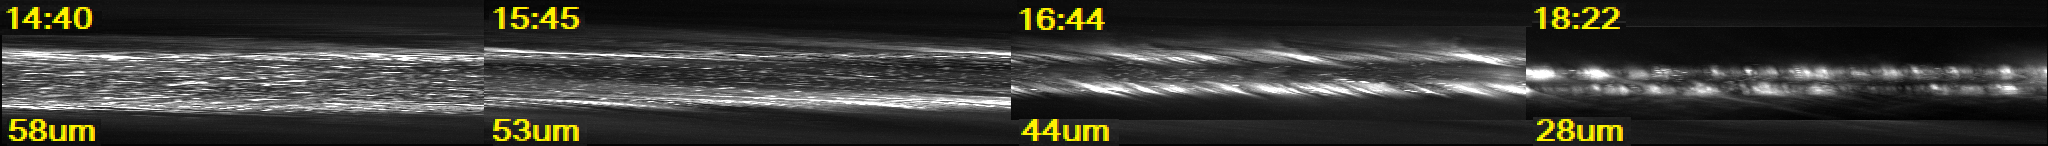
\includegraphics[width=\textwidth]{archivos/ThicknessEvolution.png}
	\caption{Evolution of the cross section of a film (time and thickness specified). Images obtained by fluorescence.}
	\label{thickness}
\end{figure}

The second option is to use the microscope to do a series of tomographies (with natural light or fluorescence), which would allow us to reconstruct the film in 3D (see Fig. \ref{thickness}). This technique is too slow, so, instead we used the focus knob to estimate the position of the bottom and the top of the layer (i.e. the position of the first and last tracers in focus)\footnote{The real thickness is not a direct output of this measurement. The procedure to obtain this value is explained in ¿¿¿ Materials and Methods ???}. In Fig. \ref{evap_rate} we can see the results of these measurements for an experiment where the box is closed with a wet cotton inside:

\begin{figure}[H]
	\centering
	\includegraphics[width=0.7\textwidth]{archivos/EvapRate.png}
	\caption{Cross section of a film over time.}
	\label{evap_rate}
\end{figure}

On the basis of this measurements, the calculated evaporation rate (slope of the curve) is about $ 0.61 \mu \textrm{m/min}$. \textcolor{red}{¿¿¿ COMMENT --> Negligible or not ???}

In addition to the temporal evolution of the film thickness, Fig. \ref{thickness} illustrates that, as expected, the fluorescent beads tend to accumulate at the surfaces. A trend that, logically, becomes more pronounced over time, since this diminishes the free surface energy. As we will see later, this can be a problem, but it makes it easier to measure the thickness.

\subsection{Numerical removal}

Background flows can be seen either in the microscope images and in the trajectories resulting of particle tracking. This algorithm outputs the particle and algae positions in every frame. Knowing the frame rate of the imaging, one can build the trajectory as a function of time. An example of tracers and algae trajectories can be seen on Fig. \ref{trajectories_e3}.

\begin{figure}[H]
	\centering
	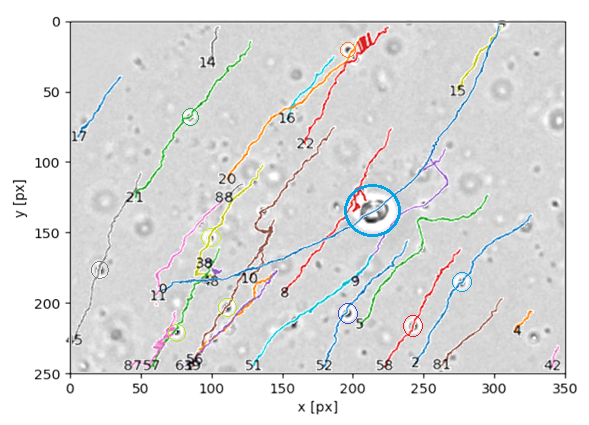
\includegraphics[width=0.8\textwidth]{archivos/trajectories_e3.png}
	\caption{Trajectories obtained by means of particle tracking superposed to one of its frames. An alga and some tracers are signaled by circles.}
	\label{trajectories_e3}
\end{figure}

The presence of a background flow, headed from the left-bottom corner to the right-top  is rather obvious on Fig. \ref{trajectories_e3}. 

Since disposing of background flows experimentally was not easy, we decided to explore the numerical removal in parallel.

Some initial ideas were put into practice and the dismissed. The main reason for this was that most of them were arbitrary in the sense that they depended on one or more subjective parameters (i.e. parameters that had to be chosen by the user). 

For instance, one of the first ideas was to split the tracers in two groups: those whose motion was affected by the presence of algae and those who were not. Once the classification done, the flow field provided by the non-affected group would be considered as the background flow and could be removed from the trajectories of the rest of the tracers.

Besides the inconvenience of having to choose a parameter whose value would determine if a bead was or not affected by the presence of algae\footnote{For this purpose we had chosen the distance to the closest alga.}, this method needed of a huge amount of tracers for the interpolation of the field to be successful. 

At this point, one might wonder where the difficulty lies when trying to remove this background flows. The beads motion is composed of three parts:

\begin{itemize}
	\item Brownian motion
	\item Motion induced by the algae 
	\item Motion induced by the background flow
\end{itemize}

Each of which is characterized by their own length and time scales. This makes it rather easy to isolate Brownian motion from the other two, because scales are very different, but when it comes to distinguish the algae contribution from the background flow, the separation is vaguer.

This is the reason why finally we decided to remove the background flow by working in a reference frame attached to the alga. The $X$ axis of this frame would be parallel to the alga's velocity vector at all times.

Since every alga behaves in a different way, this idea had an obvious problem: controlling concentration. Nonetheless, in their paper, Kurtuldu et al.~\cite{Kurtuldu2011}, explain and demonstrate experimentally that, for low levels of concentration, where one can ignore the interactions between algae (i.e. in the dilute limit), considering the tracers within a circle (with variable radius) around each alga only is equivalent to modifying concentration.  

When we speak about concentration we refer to a 2D concentration, defined as:

\begin{equation}
\Phi = \frac{n \cdot A_{alga}}{S}
\label{concentration}
\end{equation}

where $n$ is the number of algae in the image, $A_{alga}$ cross section of the alga, and $S$ is the total surface of the image.

\begin{figure}[H]
	\centering
	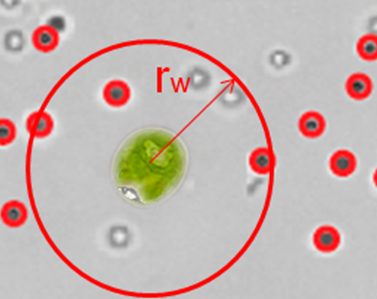
\includegraphics[width=0.4\textwidth]{archivos/concentration_circle.png}
	\caption{Specimen of \textit{Chlamydomonas reinhardtii} surrounded by tracers~\cite{chlamy_circ}. The radius of the surrounding circle determines the concentration of algae within it.}
	\label{concentration_circle}
\end{figure}

Applying this definition to the circle (see Fig. \ref{concentration_circle}) and supposing the area of an alga can be approximated by a circle whose radius is $r_{alga}$, we obtain:

\begin{equation}
\Phi = \frac{\pi r_{alga}^2}{\pi r_w^2} = \left(\frac{r_{alga}}{r_w}\right)^2
\label{conc_circle}
\end{equation}

After this small subsection, we have to focus again on the removal of the background flow by means of a change of the reference frame.

Although the Stokes number of the algae and the tracers is slightly different, we can consider that both are similarly affected by the background flow. Thus, in a mobile reference frame, background flow disappears.

Hereafter we present the pseudocode corresponding to this algorithm:

%--------------------------------------------------
\fbox{
	\begin{minipage}{15.4 cm}
		
		\vspace{0.2 cm}
		
		\textbf{Change of reference frame ¿¿¿\footnote{For further information on the classes and methods (\textit{terms in italics}), see \textcolor{red}{¿¿¿ Annex I ???}}???} 
		
		\vspace{0.2 cm}
		
		\hrule
		\vspace{0.4 cm}
		
		\textbf{Initialisation:} reading of the trajectories data (algae and tracers) and writing them on two dataframes belonging to two separate TrajectorySequence objects
		
		\vspace{0.2 cm}
		
		\textbf{Removal of the algae's Brownian motion and noise:}
		application of a \textit{derivative\_filter} to the algae trajectories
		
		\vspace{0.2 cm}
		
		\textbf{Cycle over different $\Delta t$:} repeat:
		
		\vspace{0.2 cm}
		
		\quad \textbf{Preparing parallelization:} splitting of the dataframe containing the tracer's 
		
		\quad trajectories
		
		\vspace{0.2 cm}
		
		\quad \textbf{Cycle over the existing algae:} repeat:
		
		\vspace{0.2 cm}
		
		\quad \quad \quad \textbf{Calculation of the alga direction:} we take the mean direction over $\Delta t$
		
		\vspace{0.2 cm}
		
		\quad \quad \quad \textbf{Parallel calculation of relative motion:} modulus and direction (and 
		
		\quad \quad \quad subsequent projection) of the tracers in the new frame of reference
		
		\vspace{0.2 cm}
		
		\quad \textbf{Definition of the circle around the alga} based on the desired concentration
		
		\vspace{0.2 cm}
		
		\quad \textbf{Discarding trajectories} out of the circle
		
		\vspace{0.2 cm}
		
		\quad \textbf{Saving the data} to a .csv file
		
		\vspace{0.2 cm}
		
		\textbf{Merging .csv files}
		
	\end{minipage}
}
%--------------------------------------------------

After a few attempts we obtained a clear set of images (always presenting a background flow), with a sufficient concentration of tracers and algae. This set had the particularity that the algae would behave as pushers, as it can be seen on Fig. \ref{chlamy_pusher}. 

\begin{figure}[H]
	\centering
	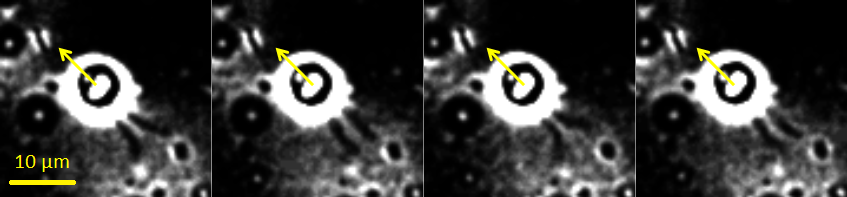
\includegraphics[width=0.8\textwidth]{archivos/chlamy_pusher.png}
	\caption{\textit{Chlamydomonas reinhardtii} behaving as a pusher (images every 0.02 seconds). The arrow indicates the direction of motion and the two flagella can be seen on the rear part of the alga.}
	\label{chlamy_pusher}
\end{figure}

This anomalous behaviour, explained in the \textcolor{red}{¿¿¿State of the art???} section, should not affect the shape of the distribution functions we are going to be looking for, but only their scales. We can, therefore, use this images to test our algorithm.

The images have been processed to improve the performance of the particle tracking algorithm (see Fig. \ref{orbpe3}). The process consists in:

\begin{figure}[H]
	\centering
	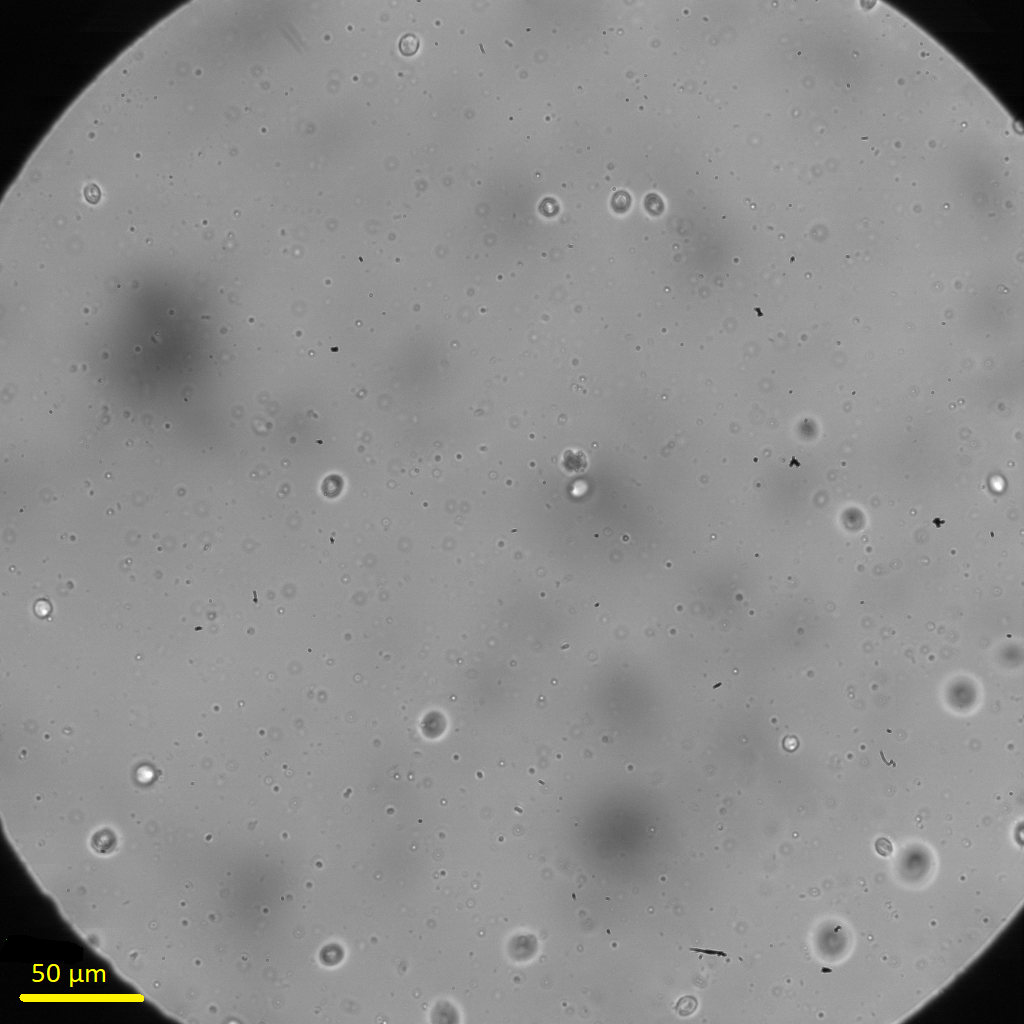
\includegraphics[width=0.4\textwidth]{archivos/frame_01_e3.png}
	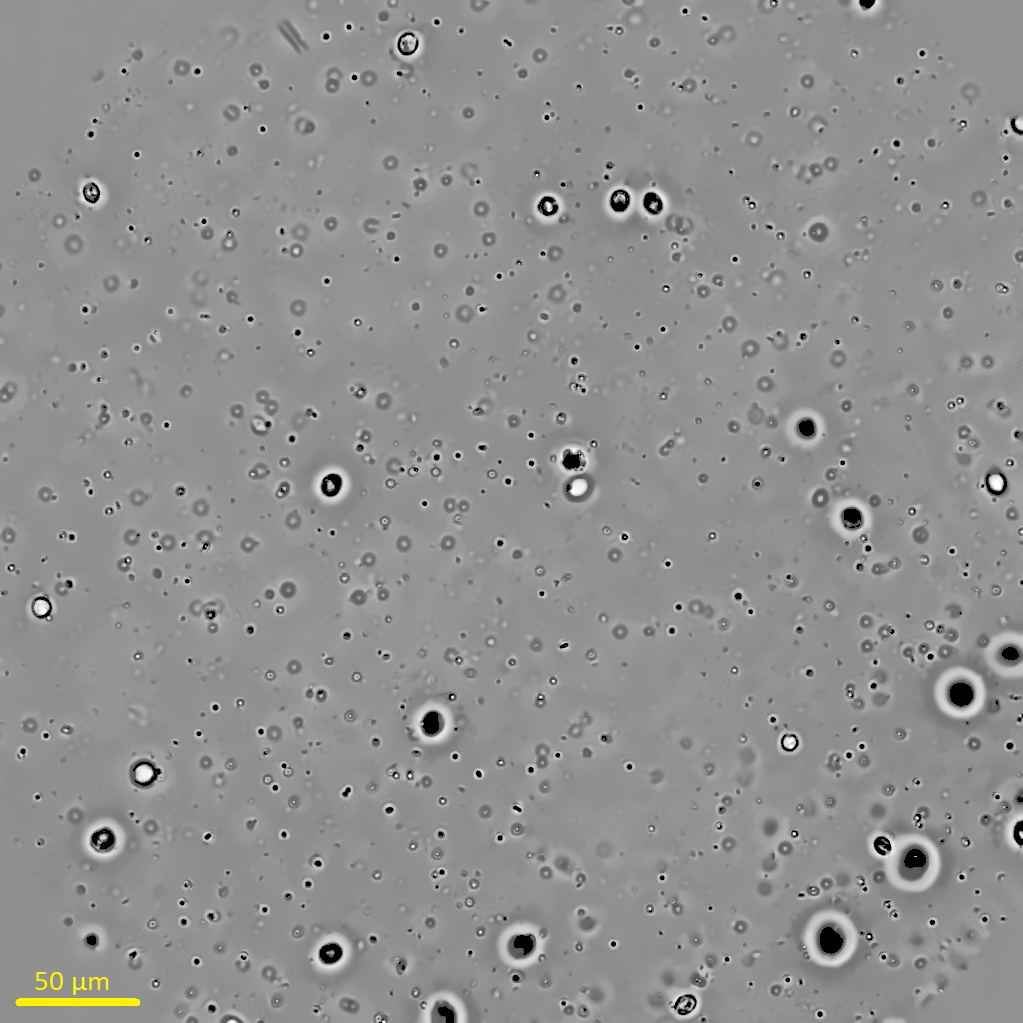
\includegraphics[width=0.4\textwidth]{archivos/frame_01_e3_bp.png}
	\caption{Original (left) and processed (right) frames.}
	\label{orbpe3}
\end{figure}

\begin{itemize}
	\item finding a mean image (over approximately 2700 frames), which is very similar to the background,
	\item removing this background of all the frames,
	\item applying a bandpass filter to highlight the structures, whose size is in the searched range,
	\item equalizing the set of images,
	\item improving contrast locally,
	\item denoising,
	\item and thresholding
\end{itemize}

Fig. \ref{prob_dist_e3} shows the probability distributions of $\Delta x$ and $\Delta y$ (in the relative frame) for a fixed $\Delta t = 0.04 \; \textrm{s}$ and a concentration\footnote{The selected concentrations result of considering circles whose diameters are: \\ 
	$ \Phi \simeq 0.3\% \rightarrow r_w = 93.03 \; \mu \textrm{m} $ \\
	$ \Phi \simeq 0.7\% \rightarrow r_w = 60.90 \; \mu \textrm{m} $ \\
	$ \Phi \simeq 2.7\% \rightarrow r_w = 31.01 \; \mu \textrm{m} $} 
$\Phi = 0.674$ :

\begin{figure}[H]
	\centering
	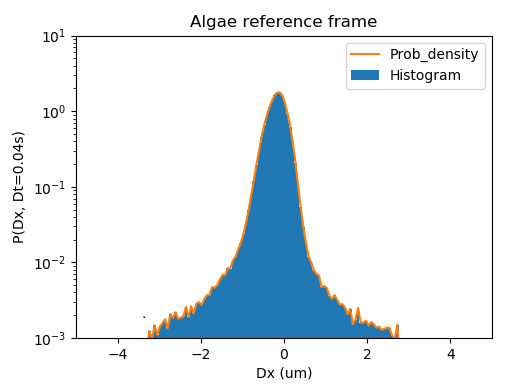
\includegraphics[width=0.42\textwidth]{archivos/pdf_x_e3.png}
	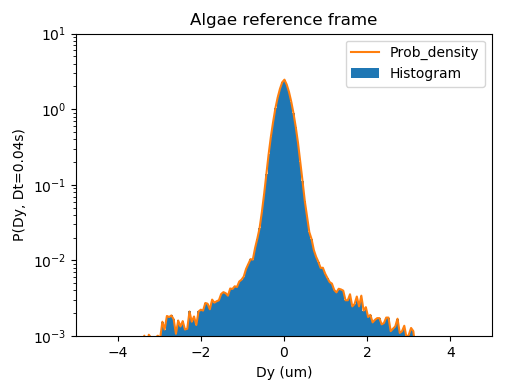
\includegraphics[width=0.4\textwidth]{archivos/pdf_y_e3.png}
	\caption{Histograms and probability distributions of the displacement $\Delta x$, (along the algae direction vector) and $\Delta y$ (perpendicular to it) in the turning reference frames attached to the algae, for a fixed $\Delta t = 0.04 \; \textrm{s}$ and $\Phi = 0.674$.}
	\label{prob_dist_e3}
\end{figure}

If background flow and algae motion were uniform, we would expect to find a $\Delta x$ distribution centered on this value (with a negative sign). In fact, reality is more complex than that and both the background flow and the velocities of the algae are subject to distribution. Even if the velocity modulus were always the same in the straight parts of the paths, the behavior of the different individuals is usually defined as a mix between \textit{run-and-tumble} and directed phototaxis~\cite{Polin}. The term \textit{run-and-tumble} describes a motion where straight paths are followed by abrupt changes in the direction of the trajectory. For this changes to occur, the modulus of the velocity goes to zero (or close to it), which partially explains the dispersion of the velocity values.

To confirm this hypothesis, one can have a look at the distributions for longer $\Delta t$ (see Fig. \ref{prob_dist_e3_longer}), where the dispersion of the algae displacements must be remarkably higher.
 
\begin{figure}[H]
	\centering
	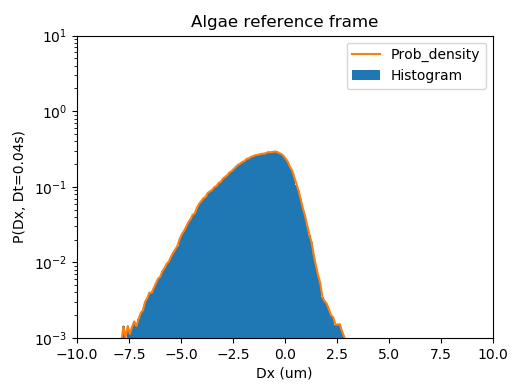
\includegraphics[width=0.42\textwidth]{archivos/pdf_x_e3_longer.png}
	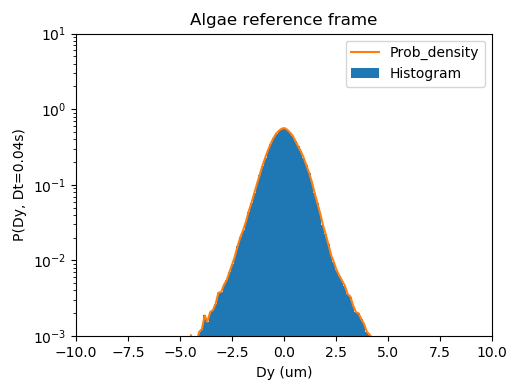
\includegraphics[width=0.4\textwidth]{archivos/pdf_y_e3_longer.png}
	\caption{Histograms and probability distributions of the displacement $\Delta x$, (along the algae direction vector) and $\Delta y$ (perpendicular to it) in the turning reference frames attached to the algae, for a fixed $\Delta t = 0.34 \; \textrm{s}$ and $\Phi = 0.674$.}
	\label{prob_dist_e3_longer}
\end{figure}

Since we ignore the distribution function of the algae velocities, let us focus on $\Delta y$. Kurtuldu et al.~\cite{Kurtuldu2011} suggest that, in the dilute limit, the probability distribution function is Gaussian, with Power Law tails. The Gaussian core corresponds to the pure Brownian motion, whereas the tails correspond to high amplitude, low probability events, that is to say, the algae kicks. 

We can fit an \textit{ad hoc} distribution to our data. The chosen distribution considers positive values only (we take the absolute value of the data) and consists of a Gaussian core, Power Law tails and a transition region. Even ignoring what the real transition law might look like, we can obtain a reasonable fitting just by imposing:

\begin{equation}
\int_{-\infty}^{\infty} f_x(x) dx = \int_{0}^{\infty} f_x(x) dx = 1
\label{probarea}
\end{equation}

where $f_x(x)$ is the probability density function, that we defined as: 

\begin{equation}
f_x(x) = \left\{
\begin{aligned}
& C_g \frac{2}{\sqrt{2 \pi \sigma^2}} e^{\frac{-x^2}{2 \sigma^2}} & \quad \textbf{if} \quad x \in [0, lim_{pl}]\\ 
& (1-m(x)^\beta) C_g \frac{2}{\sqrt{2 \pi \sigma^2}} e^{\frac{-x^2}{2 \sigma^2}} + m(x)^\beta C_{pl} (x-k)^{-\alpha} & \quad \textbf{if} \quad x \in (lim_{pl}, lim_g)\\
& C_{pl} (x-k)^{-\alpha} & \quad \textbf{if} \quad x \in [lim_g,\infty)
\end{aligned}
\right.
\end{equation}

with m(x) the transition function that we approximated as:

\begin{equation}
m(x) = \frac{x-lim_{pl}}{lim_g-lim_{pl}}
\end{equation}

On Fig. \ref{e3_adhoc} we see the results for $\sigma \simeq 0.15733 \; \mu \textrm{m}$, $lim_{pl}=0.13 \; \mu \textrm{m}$, $lim_g=0.38 \; \mu \textrm{m}$, $C_g \simeq 0.90863$, $C_{pl} \simeq 0.00386$, $k = 0$, $\beta = 2.84$, $\alpha = 5$ (values that meet the requirement expressed by Eq. \ref{probarea}).

\begin{figure}[H]
	\centering
	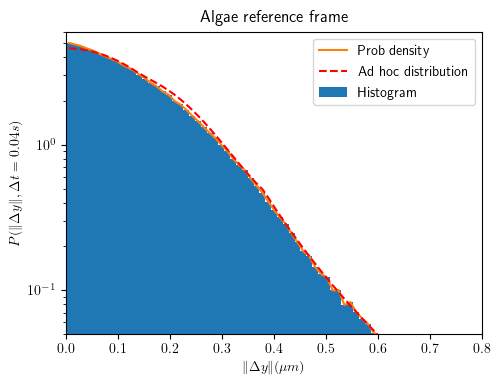
\includegraphics[width=0.4\textwidth]{archivos/pdf_ylog_e3.png}
	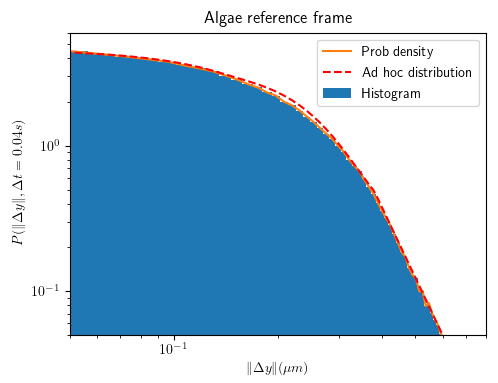
\includegraphics[width=0.4\textwidth]{archivos/pdf_loglog_e3.png}
	\caption{Fitting of the \textit{ad hoc} probability distribution function of the displacement $|\Delta y|$, (perpendicular to the algae direction vector) in the turning reference frames attached to the algae, for a fixed $\Delta t = 0.04 \; \textrm{s}$ and $\Phi = 0.674$ ($\sigma \simeq 0.15733 \; \mu \textrm{m}$, $lim_{pl}=0.13 \; \mu \textrm{m}$, $lim_g=0.38 \; \mu \textrm{m}$, $C_g \simeq 0.90863$, $C_{pl} \simeq 0.00386$, $k = 0$, $\beta = 2.84$, $\alpha = 5$)}
	\label{e3_adhoc}
\end{figure}

Regarding the results of Kurtuldu et al.~\cite{Kurtuldu2011}, we already mentioned that the scales of the distribution are affected by the studied kind of motion (pushers instead of pullers), but we also obtain a steeper descent of the Power Law tails (the exponent is $-5$ instead of $-4$). This could be logic if the energy of the kicks is lower, which seems to be the case. We will later see what happens in the case of pushers.

Another result that needs to be assessed is represented in Fig. \ref{msd_E3}. It shows the mean square tracer displacements (in the relative frame) as a function of  $\Delta t$ for different values of concentration (i.e. different circles). The mean square tracer displacement is defined as:

\begin{equation}
MSD = \frac{\displaystyle\sum_{n} \Delta x ^ 2 + \Delta y ^ 2}{n}
\end{equation}

where $n$ is the number of events. 

We are going to make the hypothesis that diffusion enhancement is isotropic (i.e. similar along $X$ and $Y$ axes). Since the motion of the algae and the background flow are ballistic along $X$ and zero in $Y$ (because of the definition of the mobile reference frame), this implies:

\begin{equation}
\Delta x = O(\Delta y) + \| \mathbf{v}_{alga} + \mathbf{v}_{bf} \| \Delta t
\end{equation}

We only want to measure diffusion, so, given the number of events is a statistically representative sample, we can write:

\begin{equation}
MSD \simeq \frac{2 \displaystyle\sum_{m} \Delta y^{2}}{n}
\label{yMSD}
\end{equation}

The MSD as defined by Eq. \ref{yMSD} is represented in Fig. \ref{MSD_e3} as a function of the elapsed time:

\begin{figure}[H]
	\centering
	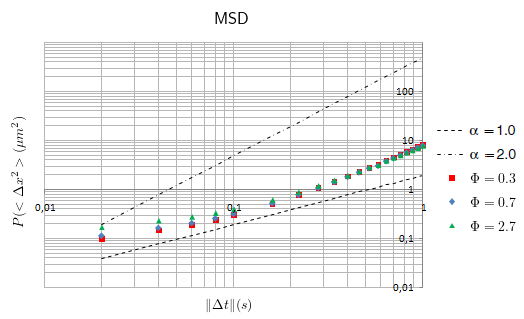
\includegraphics[width=0.6\textwidth]{archivos/MSD_e3.png}
	\caption{Mean square displacement in the turning reference frames attached to the algae as a function of $\Delta t$, for different values of $\Phi$}
	\label{MSD_e3}
\end{figure}

The behavior for $\Delta t$ under $\sim 0.1 \; \textrm{s}$ is hard to explain on a physical basis. The most plausible explanation is that, although the tracking algorithm has a theoretical precision well under the pixel ($1 \; \textrm{pixel} ~ 0.425 \; \mu \textrm{m}$), the images might be too noisy for it to work properly.

Regarding higher $\Delta t$ values, and ignoring the fact that $\Phi = 2.7\%$ is too high a concentration to be considered as belonging to the dilute limit, it is here that another problem of this methodology emerges: considering only the particles within the circles surrounding the algae may act as a filter for the long displacements. It is hard to define a cut-off length, but, since we only consider the particles that remain within a specific circle during the selected time lapse, we can say that it has to be smaller than the circle diameter. This might partially explain the convergence of the curves for different values of concentration.

As a conclusion, our numerical approach for removing the \textit{background flow} does not provide the expected results.

\section{Long-lasting films}

To summarize last section: we will set thicker films and wait for them to thin thanks to evaporation.

Just after having decided to do so, the device got damaged and we had to build a provisional one. Since we were less concerned about being precise in the initial thickness, the new device lacked of mechanisms: the threads, already in their final (stretched) position, are immersed in the solution and a film is formed between them when the device is removed vertically.

To our surprise, when the initial thickness was too high (of the order of $100 \mu \textrm m$) and, therefore, the evaporation time too long (around 1-2 hours), the algae would stop moving before we could reach the desired thickness. On the contrary, if thickness was too low, \textit{background flows} appeared again.

Several experiences were carried out to determine if the algae were dying because of a lack or excess of Oxygen or nutrients, but the results were inconclusive. 

In fact, we could not be sure if they were dying or they were only losing their flagella\footnote{In some images we appreciated detached flagella at the surface of the film. However, it is difficult to find out if algae which are not moving still have theirs.} (which can grow again in approximately one hour). The second option could have different explanations from the ones explaining death events, so it seemed appropriate to try to find out which was the case.

In order to do so, we decided to conduct a LIVE/DEAD Cell test, consisting in staining both, and which is explained in section ¿¿¿7.7???. This test did not provide the expected results for two reasons: \textit{calcein AM} seems not to be able to penetrate the algae wall, which prevents the detection of living cells; and chlorophyll is autofluorescent in the red, so it is impossible to know if we are looking at it or at \textit{EthD-1} (i.e. the dye for the dead cells, which also emits in the red spectrum).

In the end, time seemed to be more critical than thickness so, by removing the box cover in the beginning, evaporation was accelerated. Then for the last part of evaporation, the box was closed. This way, we managed to have some exploitable images without background flow and with living algae.

\section{Quiescent beads}
 
In their papers, Kurtuldu et al.~\cite{Kurtuldu2011} and Guasto et al.~\cite{Guasto} use small concentrations of surfactants to help lower the surface tension of the mixture. This facilitates the formation of the layer, whereas, theoretically, such low concentrations should not modify the general behavior of the experiment.

Nevertheless, in their article about the influence of surfactants on the drag
reduction of superhydrophobic surfaces, ¿¿¿ Peaudecerf et al.??? demonstrate that extremely low concentrations, that are present in most fluids, have huge effects on the air–liquid interface, to the point of immobilizing it. This is due to the triggering of the Marangoni effect, that is shown in the next figure:

\begin{figure}[H]
	\centering
	\includegraphics[width=0.7\textwidth]{archivos/Marangoni.png}
	\caption[Caption]{Marangoni effect in an air-water interface \textcolor{red}{¿¿¿CITE???}\protect\footnotemark caused by the presence of surfactant traces in the presence of an external flow}
	\label{Marangoni}
\end{figure}

\footnotetext{In the article, a superhydrophobic surface is represented but this does not affect the explanation.}

The presence of an external flow, which in our case could be the one generated by the breaststroke motion of the algae, generates gradients of surfactants. Since surfactants diminish the surface tension, this generates forces that oppose to this flow on the surface (Marangoni forces), altering its motion, which would, otherwise, follow that of the bulk.

This phenomena can be understood as a \textit{rigidization} of the surface, because it gives rise to parabolic velocity profiles within our layer.

All of the above could explain one of the problems we have come across during this research: some of the tracers would simply not move. Not even in a brownian way. In Fig. \ref{quiescent_beads}, we can observe some streamlines that reveal the \textit{quiescent beads}.  

\begin{figure}[H]
	\centering
	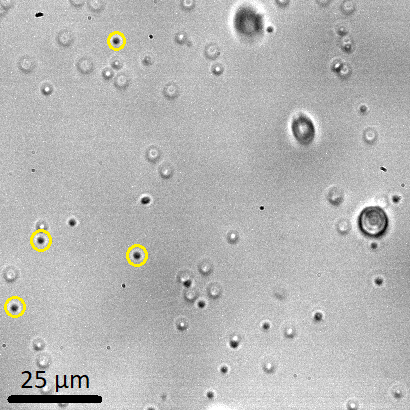
\includegraphics[width=0.4\textwidth]{archivos/190726_H2O_0_18p5um_0001.png}
	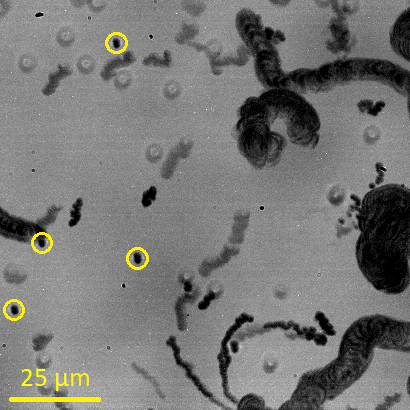
\includegraphics[width=0.4\textwidth]{archivos/190726_H2O_0_18p5um_MIN200.png}
	\caption{Quiescent beads (yellow circles) are shown in one frame (left) and its streamlines (right) for $4 \; \textrm{seconds}$ (no surfactants were added in this experiment)}
	\label{quiescent_beads}
\end{figure}

This happened in experiments where we had added no surfactant to the solution. We infer that the algal biological activity may generate some of it and, that even if it does not, it would be impossible to get completely rid of these substances.

We also know that even if the effect is not that extreme, diffusion at the interfaces is lower than in the bulk (see, for instance,~\cite{peng2009}). Moreover, our tracers will slowly sediment to the bottom interface exacerbating this trend. There does not seem to be a solution to avoid particle accumulation at the interfaces, but sedimentation can be avoided thanks to density matching. For this purpose, either  $\sim 1 \; \textrm{g/cc}$ dense spheres can be acquired or the medium can be mixed with glycerol or heavy water. Glycerol increases the viscosity of the solution, which could alter our results, so we have dismissed this option. Heavy water is probably toxic for \textit{Chlamydomonas}, but they may not be affected in the time scale of our experiment so we might consider using it in the future. Otherwise, we will try to take this factors into account when processing the data if they disturb the statistics.

\section{Last results}

After the long process described up to now in this section, we managed to get two sets of images that did not show any of the mentioned issues.

The first of them corresponds to a $\sim 20 \; \mu \textrm{m}$ thick film, and a concentration $\Phi \simeq 2.42\%$.

For long enough times, we can see that the $|\Delta x|$ distribution is almost perfectly Gaussian:

\begin{figure}[H]
	\centering
	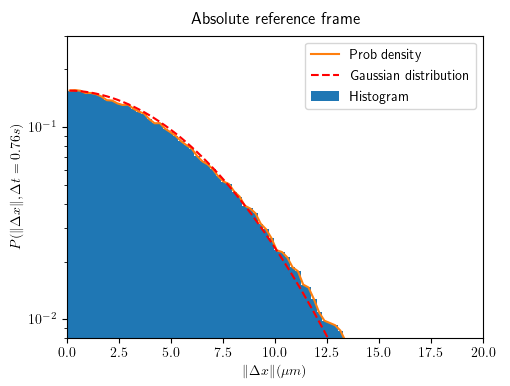
\includegraphics[width=0.4\textwidth]{archivos/GaussXpdf_ylog_Dt076_ANH_Chlamy_beads_Thickness18pt_60x.png}
	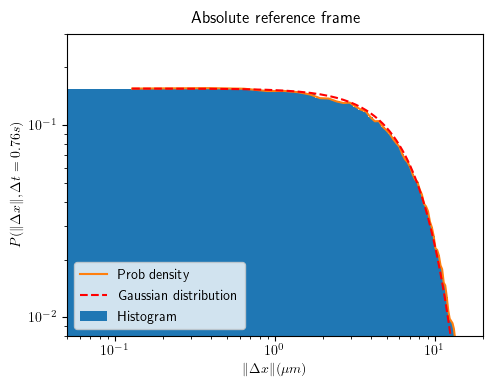
\includegraphics[width=0.4\textwidth]{archivos/GaussXpdf_loglog_Dt076_ANH_Chlamy_beads_Thickness18pt_60x.png}
	\caption{Fitting of a Gaussian to the probability distribution function of the displacement $|\Delta x|$, in the absolute reference frame, for a fixed $\Delta t = 0.76 \; \textrm{s}$ and $\Phi = 2.42\%$ ($\sigma \simeq 4.578865732063 \; \mu \textrm{m}$)}
	\label{ANH_Gauss_X}
\end{figure}

For lower times, the tails are not Gaussian anymore (see Fig. \ref{ANH_Tails}).

%\begin{figure}[H]
%	\centering
%	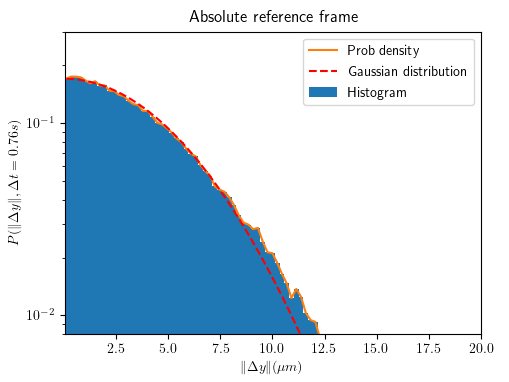
\includegraphics[width=0.4\textwidth]{archivos/GaussYpdf_ylog_Dt076_ANH_Chlamy_beads_Thickness18pt_60x.png}
%	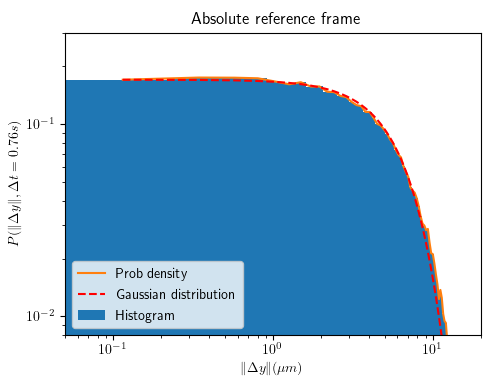
\includegraphics[width=0.4\textwidth]{archivos/GaussYpdf_loglog_Dt076_ANH_Chlamy_beads_Thickness18pt_60x.png}
%	\caption{Fitting of a Gaussian to the probability distribution function of the displacement $|\Delta y|$, in the absolute reference frame, for $\Phi = 2.42\%$ ($\sigma \simeq 5.149580504573869 \mu m$)}
%	\label{ANH_Gauss_Y}
%\end{figure}

\begin{figure}[H]
	\centering
	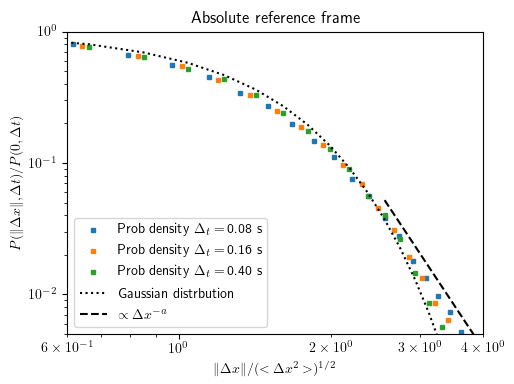
\includegraphics[width=0.6\textwidth]{archivos/TailsANH.png}
	\caption{Normalized probability distribution function of the displacement $|\Delta x|$, in the absolute reference frame, for $\Phi = 2.42\%$. The value of the exponent is $a=5.8$ for the Power Law and $\sigma \simeq 5.149580504573869 \mu m$ for the Gaussian distribution.}
	\label{ANH_Tails}
\end{figure}

As suggested by Kurtuldu et Al.~\cite{Kurtuldu2011}, tails seem to have a potential character: their slope is constant in logarithmic axes. As it can be seen on Fig. \ref{ANH_Tails}), this slope changes with  $\Delta t$, approaching the Gaussian distribution for higher values of this variable.

As we have already mentioned, the noise on the images makes it very hard to obtain valid data for $\Delta t$ under a certain threshold. This threshold's seems to be around $0.06 \; \textrm{s}$ (see Fig. \ref{MSD_ANH}). Consequently, we have only been able to measure the exponent's value for $\Delta t = 0.08 \; \textrm{s}$, which is approximately $-5.8$. This value, although far from the $-4$ obtained by Kurtuldu et Al.~\cite{Kurtuldu2011}, suggests that for lower elapsed times we can, in fact, expect something of the order of $-4$.

We can now have a look at the MSD:

\begin{figure}[H]
	\centering
	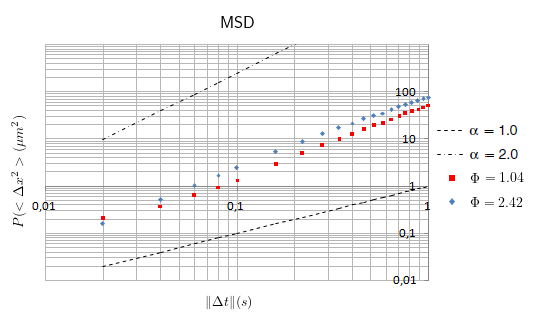
\includegraphics[width=0.6\textwidth]{archivos/MSD_ANH.png}
	\caption{Mean square displacement in the absolute reference frame as a function of $\Delta t$, for different values of $\Phi$}
	\label{MSD_ANH}
\end{figure}

The above described experiment corresponds to the blue dots, whereas the red ones have been obtained from a second exploitable set of images\footnote{Conclusions from both sets are very similar, so, for the sake of brevity, we will not further explore this data set here.}. 

We can see that the data for $\Delta t$ under $0.06 \; \textrm{s}$ draw a curve whose growth is slower than the one expected for Brownian motion. Since we can see no physical reason for this to happen, we put this error down to a precision matter, probably due to noise in the images.

Data over that threshold show a superdiffusive trend, with slopes $\sim 1.5 - 1.6$, that relax towards a normal diffusive scaling at higher values of $\Delta t$ when the distributions become Gaussian (this is more easily appreciated on the blue curve).

\textcolor{red}{¿¿¿ LOOK FOR DIFFUSION COEFS IF I HAVE THE TIME ???}
